\documentclass[oneside]{ausarbeitung}
\addbibresource{latexlit.bib}
\usepackage{todonotes} 


% ----------------------------------------------------------------------

\begin{document}

%--- Sprachauswahl
% Erlaubte Werte:
%   \selectlanguage{english}
%   \selectlanguage{ngerman}
\selectlanguage{ngerman}

%--- Art der Arbeit
% Erlaubte Werte:
%   \Praxissemesterbericht
%   \Projektbericht
%   \Bachelorarbeit
%   \Seminararbeit
%   \Masterarbeit

\Bachelorarbeit

%--- Studiengang:
% Erlaubte Werte:
%   \Informatik
%   \Elektronik
%   \DataScience
\Informatik
\title{Component-Based Web Development: Eine Revolution in der Wiederverwendbarkeit von Webkomponenten?}

\author{Jonathan Kechter}
\matrikelnr{83701}

%--- Ist der Erstbetreuer (\examinerA) an der Hochschule ein Professor?
% Erlaubte Werte:
%   \examinerIsAProfessortrue   % Ja
%   \examinerIsAProfessorfalse  % Nein
\examinerIsAProfessortrue   % Ja

%--- Betreuer
\examinerA{Prof. Dr. Carsten Lecon}
\examinerB{Sebastian Stigler}

%--- Einreichungsdatum
\date{02. April 2025}

%--- Angaben zur Firma
% Auskommentieren, wenn die Arbeit nicht bei einer ext. Firma gemacht wurde.


%--- Angaben zum Betreuer bei dieser Firma


%--- Titelseite Anzeigen
\maketitle
\cleardoublepage

%---
\pagenumbering{roman}
\setcounter{page}{1}

%--- Firmendaten Anzeigen
% Auskommentieren, wenn die Arbeit nicht bei einer ext. Firma gemacht wurde.
%\makeworkplace
\cleardoublepage

%--- Eidesstattliche Erklärung anzeigen
\makeaffirmation
\cleardoublepage

%--- Sperrvermerk (Funktioniert nur bei externen Bachelor- oder Masterarbeiten.)
%\makeconfidentialclause
\cleardoublepage

%---
\begin{abstract}
  Ziel der Kurzfassung ist es, einen (eiligen) Leser zu informieren, so 
  dass dieser entscheiden kann, ob der Bericht für ihn hilfreich ist oder 
  nicht (neudeutsch: Management Summary). Die Kurzfassung gibt daher eine 
  kurze Darstellung

  \begin{itemize}
    \item des in der Arbeit angegangenen Problems
    \item der verwendeten Methode(n)
    \item des in der Arbeit erzielten Fortschritts.
  \end{itemize}

  Dabei sollte nicht auf die Struktur der Arbeit eingegangen werden, also 
  Kapitel~\ref{cha:grundlagen} etc. denn die Kurzfassung soll ja gerade 
  das Wichtigste der Arbeit vermitteln, ohne dass diese gelesen werden muss.
  Eine Kapitelbezogene Darstellung sollte sich in Kapitel~%
  \ref{cha:einleitung} unter Vorgehen befinden.

  Länge: Maximal 1 Seite.
\end{abstract}
%-----------------------------------------------------------------------
\cleardoublepage
\tableofcontents

%---
\listoffigures

%---
\listoftables

%---
\lstlistoflistings

%---
\listofabbreviations
\begin{acronym}[Bsp.]  % Längstes Kürzel in der nachfolgenden
                       % Liste um die Breite der Spalte für die
                       % Abkürzungen zu bestimmen.

%% Eintrag: \acro{Referenzname}[Kürzel]{Langform}
%% Im Text wird die Abkürzung dann mit \ac{Referenzname} benutzt.
\acro{rup}[RUP]{Rational Unified Process}
%\acro{bsp}[Bsp.]{Beispiel}
\end{acronym}
%---


\cleardoublepage
\pagenumbering{arabic}
\setcounter{page}{1}

% ----------------------------------------------------------------------
\chapter{Einleitung}
\label{cha:einleitung}
\todo {Ausformulieren mit Fragestellung die im folgenden bearbeitet wird}
Die Einleitung dient dazu, beim Leser Interesse für die Inhalte der Bachelorarbeit zu wecken, die behandelten Probleme aufzuzeigen und die zu ihrer Lösung entwickelten Konzepte zu beschreiben.

\section{Motivation}
\label{sec:motivation}

\todo {meine motivation für die bachelorarbeit hier}

\section{Ursprünge}
\label{sec:ursprünge}
\todo {Quellen}

Die Ursprünge der Webentwicklung gehen zurück auf Tim Berners-Lee, welcher 1991 HTML, HTTP und den ersten Webbrowser entwickelte.
Recht schnell wurde klar, dass statische HTML-Seiten nicht ausreichend waren, es musste mehr Interaktivität möglich sein. Daraus entwickelte sich JavaScript, welches erstmals ermöglichte, Websites interaktiv zu machen.
Zur Trennung von Inhalt und Darstellung entstand CSS, um die visuelle Gestaltung von HTML-Seiten zu ermöglichen.
AJAX (Asynchronous JavaScript und XML) ermöglichte es erstmals, HTTP-Anfragen durchzuführen, während eine HTML-Seite dargestellt wurde, sodass die Seite aktualisiert werden konnte, ohne sie neu zu laden.
Ebenfalls wurde erstmals jQuery populär, durch die vereinfachte DOM-Manipulation und das Event-Handling.
Im Jahr 2010 folgte dann AngularJS, ein Framework, das eine MVC-ähnliche Architektur für dynamische Single-Page-Anwendungen bietet und die Entwicklung durch Two-Way Data Binding sowie modulare Komponenten erleichtert.
Im Jahr 2013 konnte React mithilfe des Virtual DOM die Performance von UI-Updates nochmal revolutionieren.
Vue.js folgte als leichtgewichtige Alternative, die einen kombinierten Ansatz aus AngularJS und React verfolgte. Es setzte auf eine einfache API, deklarative Syntax und eine reaktive Datenbindung, um eine flexible und effiziente Entwicklung zu ermöglichen.
Angular Version 2 ging auf alte Probleme ein und entwickelte ein neues, komponentenbasiertes Architekturmodell, welches sich in Komponenten, Services und Dependency Injection aufteilte. 
Im Jahr 2018 wurden Web Components als offizielle, standardisierte, frameworkunabhängige Lösung für wiederverwendbare Komponenten eingeführt.
Daraufhin stellte Svelte im darauffolgenden Jahr mit seinem neuen Konzept eines kompilierten Codes anstelle des virtuellen DOMs einen neuen Ansatz vor.

\section{Problemstellung}
\label{sec:problemstellung}

In der modernen Webentwicklung gibt es zahlreiche Frameworks und Bibliotheken, die Entwickler bei der Erstellung von Webanwendung unterstützen. Komponenten basierte Frameworks wie Angular, React und Vue.js heben sich durch ihre Modularität und Wiederverwendbarkeit von Komponenten hervor. Gleichzeitig bringen sie aber auch einige Herausforderungen mit sich. Hierzu zählt beispielsweise ein erhöhter Overhead, komplexere Buildprozesse und größere Bundle-Größen, die sich auf die Performance und Entwicklungsdauer auswirken können.
Gleichzeitig gibt es auch nicht komponentenorientierte Lösungen wie z.B. jQuery, welche durch ihre Einfachheit einen kleinere Entwicklungsprozess benötigen, dadurch aber weniger skalierbar und modular sind. 
Eine richtige technologische Entscheidung abhängig von den eigenen Bedürfnissen, bzw. denen gewünschten Projekts zu treffen, ist nicht einfach, da ein grundlegender Vergleich zwischen komponentenbasierten Ansätzen und den herkömmlichen Ansätzen fehlt. Diese Vergleiche sind oft nicht aus genügend Blickwinkeln durchgeführt worden, sondern beschränken sich auf Teilaspekte, wie die Performance, welche für eine Entscheidung nicht als einzige Metrik dienen sollte. 

\section{Abgrenzung}

Die Arbeit fokussiert sich hierbei auf die Frontendtechnologien und wird anhand eines bestimmten Implementierungsbeispiels verglichen. Hierbei wird mit folgenden Metriken gearbeitet: 
\begin{itemize}
    \item \textbf{Modularität und Wiederverwendbarkeit}:  
          Wie gut lassen sich Komponenten erstellen?
    \item \textbf{Performance und Effizienz}:  
          Wie wirken sich Frameworks auf Ladezeiten, Bundle-Größen und Rendering-Geschwindigkeit aus?
    \item \textbf{Entwicklungsaufwand und Wartbarkeit}:  
          Welche Frameworks ermöglichen eine effiziente und nachhaltige Entwicklung?
\end{itemize}

Nicht Bestandteil dieser Arbeit sind folgende Aspekte: 
\begin{itemize}
    \item \textbf{Backend-Technologien oder serverseitige Frameworks}:  
          Technologien wie Next.js, Nuxt.js oder Server-Side Rendering ermöglichen die serverseitige Verarbeitung und Darstellung von Webseiten.  
          Da der Fokus dieser Arbeit auf Frontend-Technologien liegt, werden serverseitige Lösungen nicht betrachtet.
    \item \textbf{State-Management-Lösungen innerhalb der Frameworks}:  
          Externe State-Management-Bibliotheken wie Redux, NgRx oder Vuex werden nicht untersucht, da 		der Schwerpunkt auf den Kernfunktionen der Frameworks liegt.
    \item \textbf{Full-Stack-Architekturen}:  
          Der Einfluss einer Full-Stack-Architektur auf die Wahl des Frontend-Frameworks wird nicht analysiert. Die betrachteten Frontend-Technologien werden dabei isoliert betrachtet.
    \item \textbf{Skalierung auf Großprojekte}:  
          Die Anwendbarkeit der Technologien auf groß angelegte Projekte wird nicht untersucht.  
          Eine Performance-Analyse für eine große Anzahl an Nutzern erfolgt nicht.
\end{itemize}



\section{Ziel der Arbeit}
\label{sec:ziel}

Das Ziel dieser Arbeit ist es, einen grundlegenden Vergleich zwischen verschiedenen Ansätzen in der Webentwicklung zu erstellen, den Webentwickler nutzen können, um eine fundierte Entscheidung hinsichtlich ihrer Frontendtechnologiewahl zu treffen. Der Vergleich findet zum einen grundlegend zwischen einem komponentenbasierten Ansatz sowie einem herkömmlichen Ansatz statt. Außerdem wird im Detail untersucht, inwieweit welche komponentenbasierten Frameworks Vor- und Nachteile gegenüber den anderen Lösungen haben. Der Vergleich wird anhand folgender Metriken erstellt:  

\begin{itemize}
    \item \textbf{Modularität und Wiederverwendbarkeit}:  
          Wie gut lassen sich Komponenten im Framework erstellen, und wie lassen sie sich innerhalb der Anwendung wiederverwenden, um eine modulare Architektur zu fördern und gleichzeitig Code-Dopplungen zu vermeiden?  
    \item \textbf{Performance und Effizienz}:  
          Wie wirken sich Frameworks auf Ladezeiten, Bundle-Größen und Rendering-Geschwindigkeit aus?  
          Zusätzlich wird untersucht, ob der Overhead des jeweiligen Frameworks die Performance signifikant beeinträchtigt.  
    \item \textbf{Entwicklungsaufwand, Wartbarkeit und Erweiterbarkeit}:  
          Welche Frameworks ermöglichen eine effiziente und nachhaltige Entwicklung?  
          Zusätzlich wird untersucht, ob die Anwendung leicht erweitert werden kann, indem neue Funktionen hinzugefügt oder bestehende Module angepasst werden.  
          Außerdem wird untersucht, ob die Architektur des Frameworks für größere Nutzerzahlen skalierbar wäre bzw. komplexere Anwendungen unterstützt.  
\end{itemize}

\section{Vorgehen}
\label{sec:vorgehen}

Das Vorgehen der Arbeit ist in mehrere strukturierte Abschnitte unterteilt, die in den folgenden Kapiteln behandelt werden. Hierbei wird auf Basis der Grundlagen und der vorgestellten Problemstellung gezielt auf die Lösung hingearbeitet. 
Das komplette Vorgehen lässt sich in folgende Kapitel aufteilen: 

\todo {Ausformulieren sobald alle Kapitel stehen}
\begin{enumerate}  
	\item \textbf{Grundlagen Kapitel 2}: Hier wird auf alle relevanten technischen und theoretischen Konzepte der Arbeit eingegangen um ein gleichen Wissensstand zu garantieren. Das Kapitel befasst sich mit allen Frontendtechnologien sowie mit der Komponentenbasierten Architektur um ein grundlegendes Verständnis für das folgende Kapitel zu schaffen. 
    \item \textbf{Problemanalyse (Kapitel 3)}: 
    \item \textbf{Lösungskonzept (Kapitel 4)}: 
    \item \textbf{Implementierung (Kapitel 5)}: 
    \item \textbf{Evaluierung (Kapitel 6)}:   
    \item \textbf{Zusammenfassung und Ausblick (Kapitel 7)}:	
\end{enumerate}  
% ---
\chapter{Grundlagen}
\label{chap:grundlagen}

% Einführung in das Kapitel
Im folgenden Kapitel werden alle technologischen Grundlagen der Arbeit dargestellt.
 
\section{TypeScript}
Typescript ist eine von Microsoft entwickelte Programmiersprache, welche auf JavaScript basiert. Sie erweitert JavaScript um eine statische Typisierung, wodurch Fehler schon während der Entwicklung erkannt werden können und verringert dadurch die Anzahl an Laufzeitfehlern. Typescript Code wird in normales JavaScript konvertiert und kann dadurch in allen JavaScript Umgebungen verwendet werden, wie z.B. Browsern, Node.js\footnote{https://nodejs.org/en} und Deno\footnote{https://docs.deno.com/runtime/} (vgl. \parencite{typescript}). 

\section{Supabase}
\subsection{Allgemeines}
Supabase ist eine Open-Source-Alternative zu Firebase. Es handelt sich um eine PostgreSQL-Datenbanklösung, die Datenbank, Authentifizierung, Storage und Serverless Functions auf einer zentralen Plattform vereint. Jede Supabase-Instanz basiert auf einer vollwertigen PostgreSQL-Datenbank, die mithilfe von Row Level Security (RLS) eine sichere Datenverwaltung garantiert (vgl. \parencite{supabase}).

\subsection{Authentifizierung}
Die Authentifizierung von Supabase unterstützt E-Mail/Passwort, OAuth, Magic Links sowie eine große Auswahl an Social Logins. Mithilfe von WebSockets ermöglicht Supabase die Umsetzung von Echtzeit-Funktionalitäten (vgl. \parencite{supabase}).

\subsection{Storage und REST-API}
Zudem bietet die Plattform einen integrierten Storage, der das Speichern und Verwalten großer Dateien wie Videos und Bilder erleichtert. Durch fertige RESTful APIs können Entwickler direkt auf die Datenbank zugreifen und CRUD-Operationen (Create, Read, Update, Delete) durchführen, ohne zusätzlichen Backend-Code schreiben zu müssen (vgl. \parencite{supabase}). 

\section{Node.js}
\subsection{Allgemeines}
Node.js ist eine kostenlose, Open-Source, cross-platform JavaScript-Laufzeitumgebung, die es einem ermöglicht, Server, Web-Apps, Kommandozeilen-Tools oder Scripts zu erstellen. Node.js basiert auf der V8-Engine von Google Chrome, welche JavaScript in Maschinencode kompiliert, wodurch es eine sehr effiziente Lösung ist (vgl. \parencite{nodejs}).

\subsection{Architektur}
Node.js-Apps laufen in einem einzelnen Prozess, ohne für weitere Anfragen neue Threads zu erstellen. Bei I/O-Operationen blockiert Node.js keine Threads, sondern lässt diese weiterlaufen, sobald eine Antwort zurückkommt. Dadurch kann Node.js tausende von nebenläufigen Verbindungen auf einem einzelnen Server aufrechterhalten, ohne sich um das Verwalten von Threads zu kümmern (vgl. \parencite{nodejs}).

\subsection{Vorteile für Entwickler}
Ein großer Vorteil besteht außerdem für Frontend-Entwickler, welche im Frontend bereits JavaScript nutzen und ihre Kenntnisse auch im Backend anwenden können, ohne eine neue Sprache lernen zu müssen. Dadurch wird ein schnellerer Einstieg ermöglicht (vgl. \parencite{nodejs}).

\section{npm (Node Package Manager)}
\subsection{Allgemeines}
npm ist die weltweit größte Software-Registry für Open-Source-Entwicklung. Mit npm kann man JavaScript-Pakete verwalten und teilen wodurch sie weltweit von Entwicklern genutzt werden können (vgl. \parencite{npm}). 

\subsection{Hauptkomponenten}
npm besteht aus den drei Hauptkomponenten: Website, CLI und Registry. Die Website ermöglicht die Verwaltung und Entdeckung von Paketen. Das CLI ermöglicht die Nutzung über das Terminal, und die Registry stellt eine zentrale Datenbank für alle Pakete dar (vgl. \parencite{npm}).

\subsection{Versionierung und Organisation}
Mit npm lassen sich Versionen und Abhängigkeiten verwalten sowie automatische Updates einstellen. Für Entwickler besteht die Möglichkeit, eine npm-Organisation zu erstellen, die es ermöglicht, Pakete gemeinsam zu verwalten und dabei Code-Restriktionen durch Berechtigungen in Teams zu erstellen (vgl. \parencite{npm}).

\section{npx (Node Package Execute)}
\section{npx (Express)}
\section{npx (Corse)}

\section{Frontend-Technologien}

\subsection{Angular}
Angular ist ein auf TypeScript basierendes Web-Framework, das von Google entwickelt wurde. 

\subsubsection{Struktur und Komponenten}
Angular bietet ein breites Angebot an Werkzeugen, APIs und Bibliotheken, durch die der Entwicklungsprozess vereinfacht werden soll. Durch Hilfe von Angular Komponenten kann der Code während der Entwicklung in verkapselte Module unterteilt werden (vgl. \parencite{angular}).

\subsubsection{State Management und Routing}
Mit Signals lassen sich State-Updates einfach in die Anwendung einbinden, wodurch eine schnelle Aktualisierung bei Änderungen ermöglicht wird. Mithilfe der Angular-Routing-Struktur lassen sich Navigationen mit Route Guards, Data Resolutions und Lazy Loading einfach umsetzen (vgl. \parencite{angular}).

\subsubsection{Entwicklungstools}
Mit der Angular CLI lassen sich Projekte innerhalb einer Minute aufsetzen und Komponenten, Services etc. direkt im Terminal generieren. Die Angular DevTools können als Erweiterung der im Browser bereits vorhandenen Entwickler-Tools genutzt werden und helfen dabei, die App zu analysieren – mithilfe von Komponentenbaum-Inspektoren, Dependency Injection Trees und angepassten Performance-Diagrammen (vgl. \parencite{angular}).

\subsection{React}
React ist eine von Meta entwickelte JavaScript-Bibliothek, die zur Erstellung von Benutzeroberflächen für Web- und native Anwendungen genutzt werden kann.

\subsubsection{Komponentenbasierte Architektur}
Mithilfe einer komponentenorientierten Architektur ist es möglich, mit React das User Interface aus wiederverwendbaren Komponenten aufzubauen. Eine React-Komponente ist eine eigenständige JavaScript-Funktion, die UI-Elemente zurückgibt (vgl. \parencite{react}).

\subsubsection{JSX und Event Handling}
Hierbei wird JSX (JavaScript XML) genutzt, welches es erleichtert, durch eine Mischung aus HTML und JavaScript React-Komponenten zu erstellen, aufrechtzuerhalten und zu löschen. Die Interaktion des Users mit Komponenten wird über Event Handling ermöglicht, wobei onClick und onChange häufig genutzte Ereignisse sind (vgl. \parencite{react}).

\subsubsection{State Management}
Daten lassen sich zwischen Komponenten über Props übergeben, wodurch übergeordnete Komponenten Informationen an untergeordnete Komponenten weitergeben können. Mithilfe von useState lassen sich lokale Zustände innerhalb einer Komponente verwalten, während useEffect verwendet wird, um Seiteneffekte innerhalb einer Komponente auszuführen (vgl. \parencite{react}).

\subsection{Web Components}
Web Components sind eine Sammlung von Technologien, die zur Erstellung wiederverwendbarer UI-Komponenten genutzt werden können (vgl. \parencite{webcomponents}). 

\subsubsection{Erstellung und API}
Mithilfe von JavaScript-APIs ist es möglich, eigene benutzerdefinierte Elemente zu erstellen. Die Definition einer Komponente mit einem eigenen HTML-Tag erfolgt mit CustomElementRegistry.define(). Eine Komponente durchläuft einen Lebenszyklus, beginnend mit connectedCallback(), welches aufgerufen wird, wenn das Element ins DOM eingefügt wird. Bei Änderungen an Attributen erfolgt attributeChangedCallback(), während disconnectedCallback() ausgeführt wird, wenn das Element aus dem DOM entfernt wird (vgl. \parencite{webcomponents}).

\subsubsection{Shadow DOM}
Durch den per JavaScript-API bereitgestellten Shadow DOM ist es möglich, eine gekapselte DOM-Struktur innerhalb einer Web-Komponente zu erstellen. Dadurch wird verhindert, dass Stil- und Skript-Konflikte zwischen den Komponenten und der Hauptseite entstehen (vgl. \parencite{webcomponents}).

\subsubsection{Styling}
Mithilfe von \texttt{<template>} und \texttt{<slot>} besteht die Möglichkeit, wiederverwendbare HTML-Templates zu erstellen, die dynamisch eingefügt werden können. Für das passende CSS-Styling der erstellten Komponenten besteht die Möglichkeit, mit \texttt{:host} Stile direkt auf benutzerdefinierte Elemente anzuwenden. Ebenfalls kann per \texttt{:host-context()} CSS-Regeln an den Kontext des Elements angepasst und mit \texttt{::slotted()} das Styling von Inhalten aus Slots beeinflusst werden (vgl. \parencite{webcomponents}).


\subsection{jQuery}
jQuery ist eine leichtgewichtige JavaScript-Bibliothek, die zur DOM-Manipulation, Event-Steuerung und Animationen verwendet werden kann (vgl. \parencite{jquery_api}).  
Mithilfe von jQuery können einfachere und kürzere JavaScript-Befehle im Vergleich zu Vanilla JavaScript verwendet werden (vgl. \parencite{jquery-api}).  

\subsubsection{Einbindung von jQuery}
jQuery kann lokal über das \texttt{\textless script\textgreater}-Tag eingebunden werden und muss dabei auf eine Kopie von jQuery oder eine Version mit Versionsnummer verweisen (vgl. \parencite{jquery_api}).  

\subsubsection{DOM-Manipulation mit jQuery}
jQuery ermittelt mithilfe von \texttt{\$(document).ready()}, dass der Code erst nach vollständigem Laden des DOMs ausgeführt wird. Die Funktion \texttt{ready} signalisiert hierbei, dass das Dokument bereit ist, um mithilfe des DOMs manipuliert zu werden (vgl. \parencite{jquery_api}).  

\subsubsection{Event Handling in jQuery}
Events wie Klicks auf Buttons oder Links können direkt an Elemente angebunden werden. Ihr Verhalten kann hierbei entsprechend angepasst werden. Mithilfe von  
\texttt{event.preventDefault()} lässt sich das Standardverhalten eines Links oder Buttons verhindern (vgl. \parencite{jquery_api}).  

\subsubsection{Dynamisches CSS mit jQuery}
jQuery bietet auch die Möglichkeit, CSS-Klassen dynamisch zu verwalten.  
CSS-Klassen können mithilfe von \texttt{.addClass("class-name")} hinzugefügt bzw. mit \texttt{.removeClass("class-name")} entfernt werden (vgl. \parencite{jquery_api}).  

\subsubsection{Effekte und Animationen}
Für Verfeinerungen lassen sich mit jQuery auch Effekte und Animationen in die Anwendung hinzufügen. Hierbei lässt sich z. B. mit \texttt{.hide()} oder \texttt{.show()} etwas ausblenden bzw. einblenden (vgl. \parencite{jquery_api}).  

\subsubsection{Callbacks und asynchrone Verarbeitung}
Mithilfe von Callbacks lassen sich Funktionen als Argumente an eine andere Funktion übergeben. Sie werden erst dann ausgeführt, wenn die übergeordnete Elternfunktion vollständig verarbeitet wurde. Dadurch lassen sich asynchrone Operationen steuern, wie beispielsweise das Laden einer HTML-Datei mithilfe von \texttt{\$.get()}. Erst nach Abschluss des Ladevorgangs wird die Callback-Funktion aufgerufen.  

\begin{lstlisting}[language=Java, caption={Verwendung eines Callbacks in jQuery}]
$.get("myhtmlpage.html", function() { 
    myCallBack(param1, param2); 
});
\end{lstlisting}

In diesem Beispiel wird die Funktion \texttt{myCallBack(param1, param2)} erst dann ausgeführt, wenn der Inhalt der Datei \texttt{myhtmlpage.html} erfolgreich geladen wurde. Dadurch wird sichergestellt, dass die abhängige Verarbeitung erst nach Abschluss des Ladevorgangs beginnt (vgl. \parencite{jquery_api}).  


\section{Zusätzliche Werkzeuge}

\subsection{LaTeX}
\todo {Ausformulieren}
- Dokumentenerstellungssystem für wissenschaftliche Arbeiten  
- Ermöglicht strukturierte und professionelle Formatierung  
- Nutzung für die Erstellung der Bachelorarbeit  

\subsection{Git}
\todo {Git kürzen!}

Git ist ein verteiltes Versionsverwaltungssystem, welches die gemeinsame Verwaltung von Quellcode über mehrere Nutzer und Geräte möglich macht.  

\subsubsection{Snapshots statt Dateiunterschiede}
Im Vergleich zu anderen Versionierungssystemen arbeitet Git mit \texttt{Snapshots} anstatt mit Dateiunterschieden. Hierbei wird eine vollständige Abbildung des ganzen Projekts erstellt und eine entsprechende Referenz gespeichert. Dabei werden Dateien, die keine Änderungen enthalten, nicht dupliziert, sondern es wird auf die ältere Version verwiesen (vgl. \parencite{git_intro}).  

\subsubsection{Arbeiten ohne Internetverbindung}
Nutzer müssen sich keine Gedanken über eine bestehende Internetverbindung machen, da Git größtenteils offline genutzt werden kann. Dateien können somit schon früher \texttt{committed} werden und anschließend später, bei wieder bestehender Internetverbindung, \texttt{gepusht} werden (vgl. \parencite{git_intro}).  

\subsubsection{Datensicherheit und Wiederherstellung}
Sobald eine Änderung an einer Datei \texttt{committed} wurde, ist es ziemlich schwer, diese Änderung anschließend mit Git wieder zu verlieren, da Git zum Großteil bei allen Operationen nur Daten zur Git-Datenbank hinzufügt. Jeder Zustand während der Entwicklung kann somit rückblickend verfolgt und wiederhergestellt werden, wodurch man sich keine Gedanken machen muss, neue Dinge auszuprobieren – selbst wenn diese fehlschlagen, da man jederzeit den alten Stand wiederherstellen kann (vgl. \parencite{git_intro}).  

\subsubsection{Die drei Zustände einer Datei}
Bei der Arbeit mit Git können sich Dateien in drei verschiedenen Zuständen befinden: \texttt{modified}, \texttt{staged} und \texttt{committed}.  
\texttt{Modified} bedeutet, dass die Datei geändert wurde, aber noch nicht auf die Datenbank \texttt{committed} wurde.  
\texttt{Staged} bedeutet, dass die Datei geändert wurde und für den nächsten \texttt{Commit} markiert wurde.  
\texttt{Committed} bedeutet, dass die Datei auf die lokale Datenbank \texttt{committed} wurde. (vgl. \parencite{git_intro})

\subsubsection{Branches in Git}
Git ermöglicht mithilfe von Branches, parallel an verschiedenen Dingen zu arbeiten. Branches können genutzt werden, um Änderungen zu testen und anschließend problemlos wieder zum ursprünglichen Branch zu wechseln, um dort weiterzuarbeiten oder die gewünschten Änderungen in den aktuellen Branch zu mergen (vgl. \parencite{git-branching-merging}).  

\subsubsection{Branching-Strategien}
Es können außerdem Strukturen entworfen werden, die die Entwicklung einer Anwendung in verschiedene Bereiche unterteilen. So kann ein Branch den aktuellen produktiven Stand darstellen, während ein anderer den neuesten Entwicklungsstand enthält. Zur Entwicklung neuer Funktionen können Branches speziell für die Implementierung einzelner Features erstellt werden (vgl. \parencite{git-branching-merging}).


\subsection{Sourcetree}
Sourcetree ist eine grafische Benutzeroberfläche für \texttt{Git}, in der alle \texttt{Git}-Kommandos einfach ausgeführt werden können. \texttt{Sourcetree} unterstützt den Nutzer bei allen relevanten \texttt{Git}-Aktionen wie \texttt{commits}, \texttt{pulls}, \texttt{pushes} usw., ohne dass die entsprechenden Befehle erlernt werden müssen. Auch komplexere Aktionen wie \texttt{changesets}, \texttt{stash} und \texttt{cherry-pick} können bequem über die Anwendung ausgeführt werden.
Alle Änderungen, die an Dateien vorgenommen wurden, werden visuell eindeutig und farblich hervorgehoben dargestellt. Dadurch lassen sich vor einem \texttt{commit} alle Änderungen nochmals überprüfen.
Alle \texttt{commits} mit den zugehörigen \texttt{branches} werden grafisch in Form einer \texttt{Commit}-Historie dargestellt, sodass alle Code-Änderungen auf einen Blick ersichtlich sind.
Bei der Nutzung im Team bietet \texttt{Sourcetree} \texttt{branching}-Diagramme, die den Entwicklungsprozess des Teams veranschaulichen, um eine bessere Übersicht über die aktuelle Entwicklung zu ermöglichen \parencite{sourcetree}. 

\subsection{VS Code}
Visual Studio Code ist ein kostenloser, plattformübergreifender Code-Editor, der zahlreiche Programmiersprachen und Erweiterungen unterstützt. Diese helfen dem Nutzer bei der Entwicklung durch Funktionen wie \texttt{Syntax-Highlighting}, \texttt{Auto-Completion} und \texttt{Linting}.
Es bietet außerdem eine integrierte Unterstützung für die Versionsverwaltung mit Git. Damit können Repositorys und Branches erstellt sowie Commits, Pushes usw. durchgeführt werden.
Visual Studio Code verfügt über ein integriertes Debugging-Tool, mit dem Breakpoints gesetzt, Variablen inspiziert und Schrittweises Debugging durchgeführt werden kann.
IntelliSense ist eine intelligente Code-Vervollständigung, die abhängig vom Kontext und installierten Erweiterungen passenden Code zur Vervollständigung vorschlägt \parencite{vs-code}.

\section{Zusammenfassung}
\todo {Ausformulieren}
- Beschreibung der verwendeten Technologien  
- TypeScript als Programmiersprache für das Backend  
- Vergleich verschiedener Frontend-Technologien hinsichtlich Modularität und Wiederverwendbarkeit  
- Supabase als zentrale Lösung für Datenbank und Authentifizierung  
- Nutzung von Git und Sourcetree für Versionskontrolle  
- LaTeX für die Dokumentation der Arbeit  
- VS Code als zentrale Entwicklungsumgebung  

%---
\chapter{Problemanalyse}
\label{cha:problemanalyse}

\section{Einleitung}
Die moderne Webentwicklung setzt vermehrt auf komponentenbasierte Architekturen, wozu eine Vielzahl an verschiedenen Frameworks existiert, die diese Architektur auf verschiedene Weisen umsetzen. Frameworks wie React, Next.js und Angular gehören zu den meistgenutzten Frameworks, während nicht-komponentenbasierte Ansätze wie jQuery immer weniger vertreten sind (vgl. \parencite{statista2024}).
\begin{figure}[h]
    \centering
    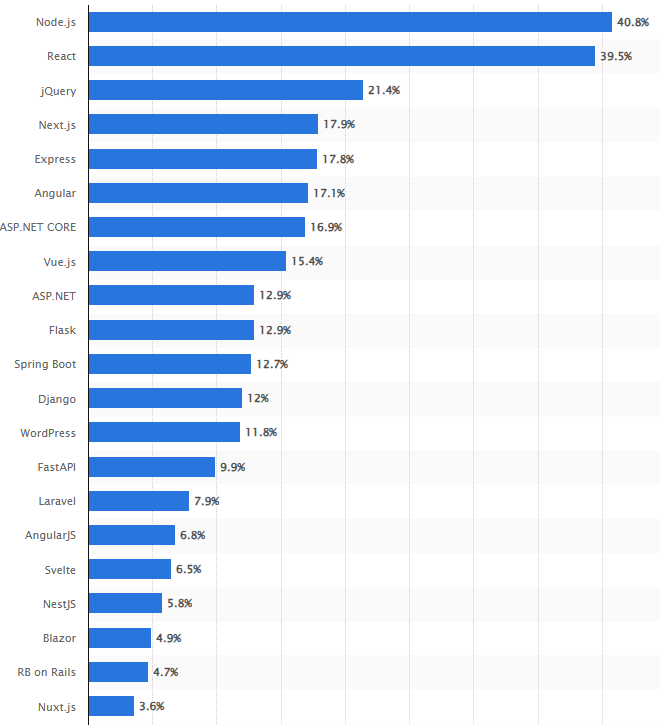
\includegraphics[width=0.8\textwidth, height=0.5\textheight, keepaspectratio]{images/web-frameworks.png}
    \caption{Meistgenutzte Web-Frameworks weltweit (Quelle: Statista)}
    \label{fig:frameworks}
\end{figure}

Bei der Auswahl eines passenden Frameworks fehlt jedoch ein ausgiebiger Vergleich hinsichtlich verschiedener Metriken. Im folgenden Kapitel wird dargestellt, warum ein solcher neuer, umfassender Vergleich notwendig ist.

\section{Aktuelle Situation in der Webentwicklung}
\todo {Überarbeiten größere Blöcke und Zitate zsm fassen}
Die Webentwicklung zeigt einen klaren Trend in Richtung komponentenbasierter Ansätze für die Frontend-Entwicklung mithilfe von Frameworks wie Angular, React und Vue (vgl. \parencite[S. 44]{js-framework-comparison}). 

Alle Frameworks legen ihren Fokus auf wiederverwendbare Komponenten, um die Modularität, Wartbarkeit und Skalierbarkeit der Anwendungen zu steigern (vgl. \autocite [S. 7]{spa-frameworks-2024}). 

Alle Frameworks haben ihre Vor- und Nachteile, zeichnen sich aber oft durch einen gewissen Overhead durch die eingebaute Komplexität aus. Angular bietet hierbei eine große Skalierbarkeit, während React für komplexe User Interface Elemente sinnvoll ist und Vue.js sich durch durch die Einfachheit für kleinere Anwendungen auszeichnet (vgl. \parencite[S. 4]{frontend-frameworks-comparison}). 

Der Entwicklungsaufwand sowie die Wartbarkeit von komponentenbasierten Frameworks kann mit steigender Anwendungsgröße immer komplexer werden. Bei nicht ausreichender Architekturplanung kann eine große technische Schuld entstehen, wie durch die tief verschachtelten Komponentenbäume in React, welche eine Wartbarkeit stark erschweren können (vgl. \parencite[S. 29]{comparison-frameworks-scalable-apps}).
\todo{quelle finden!}
Die Performance der Frameworks variiert hinsichtlich ihres Ansatzes, wodurch React und Vue durch die Nutzung eines Virtual DOMs wesentlich schneller bei der Aktualisierung von Elementen sind als Angular und Svelte (vgl. \parencite[S. 61]{js-framework-comparison}).

Trotz einer verbreiteten Nutzung der Frameworks gibt es keinen umfassenden Vergleich. Diese Defizite werden im folgenden Abschnitt genauer aufgezeigt. 

\section{Forschungsstand und bestehende Vergleiche}
\subsection{Vorhande Vergleichsstudien}
Der aktuelle Forschungsstand bringt einzelne Vergleiche, welche aber nur auf Teilaspekte eingehen. Hier eine Sammlung der bereits vorhandenen Ergebnisse: 
\begin{itemize}
    \item \textbf{Performance-Vergleich}: Frameworks wie React und Vue mit der Virtual DOM zeigen einen Vorteil durch schnellere Updates, haben aber einen erhöhten Speicherverbrauch. Angular nutzt die Incremental DOM, welche langsamer ist, aber dadurch strukturierter für große Anwendungen ist. Svelte besitzt keinen Virtual DOM, wodurch kompakte Builds mit weniger Flexibilität erstellt werden können \parencite[S.61]{js-framework-comparison}
	\item \textbf{Skalierbarkeit und Wartbarkeit}: Angular fördert die Entwicklung wiederverwendbarer, modularer Komponenten, wodurch mithilfe von TypeScript eine zusätzliche Struktur entsteht. Dies ermöglicht es großen Teams, skalierbare Anwendungen mit passenden Interfaces und Services zu erstellen. Mit zunehmender Größe der Anwendung wird die Wartbarkeit jedoch immer schwieriger. In Frameworks wie React besteht schnell die Gefahr, dass der Komponentenbaum zu tief verschachtelt wird, wodurch die Verfolgung der Datenübertragung immer schwerer wird \parencite[S. 25,28]{comparison-frameworks-scalable-apps}.
    \item \textbf{Modularität und Wiederverwendbarkeit}: Angular fördert die Entwicklung von modularen, wiederverwendbaren Komponenten. Diese sind mithilfe von Typescript klar definiert und erleichtern die Strukturierung großer Anwendungen. React bietet ebenfalls eine modulare Struktur, durch welche Komponenten über die ganze Anwendung hinweg wiederverwendbar sind. Durch eine horizontale Skalierung können komplexe React UI in kleine, einfache Komponenten aufgeteilt werden. Vue.js Komponenten sind klein, eigenständig und wiederverwendbar aufgebaut und können dann zum Zusammenbau größerer komplexerer Module verwendet werden \cite[S. 24,26] {comparison-frameworks-scalable-apps}.
    
\end{itemize}

\section{Notwendigkeit eines neuen Vergleichsansatzes}

Die bestehenden Vergleiche fokussieren sich oft nur auf bestimmte Aspekte, wie die Rendering Performance oder Bundle-Größen. Dies sind wichtige Metriken, decken aber nur einen Teilaspekt ab. Hier ist eine ganzheitliche Betrachtung nötig, die auch den Entwicklungsaufwand, die Wartbarkeit sowie Skalierbarkeit berücksichtigt. Bisherige Vergleiche nutzen hauptsächlich Benchmarks und vergleichen anhand dieser die Frameworks. Für eine größere Vergleichsabdeckung ist ein Vergleich der Frameworks bei Nutzung in einem echten Nutzerszenario nötig. 

\section{Zusammenfassung der Problemstellung}
\todo{überarbeiten klingt ähnlich wie vorheriges kapitel}
Der ansteigende Einsatz von komponentenbasierten Frameworks wie React, Angular, Vue und weiteren bietet viele Vorteile hinsichtlich Wiederverwendbarkeit und Modularisierung. Jedoch entstehen auch Herausforderungen hinsichtlich des Entwicklungsaufwands, der Code-Komplexität und der langfristigen Wartbarkeit.

Das Problem der Arbeit ergibt sich aus einer Lücke, die bei bisherigen Vergleichen von komponentenbasierten Frameworks besteht. Diese konzentrieren sich oft nur auf spezifische Metriken wie Ladezeiten und stellen dadurch keinen umfassenden Vergleich dar.

Diese Arbeit schließt diese Lücke, indem sie auf eine ganzheitliche Analyse eingeht, die neben Performance-Metriken auch Skalierbarkeit, Wartbarkeit und den tatsächlichen Entwicklungsaufwand untersucht. Der Vergleich erfolgt anhand einer realen Anwendung, um die Frameworks nicht nur unter theoretischen Aspekten, sondern auch in einem praxisnahen Nutzerszenario zu bewerten.

%---
\chapter{Lösungskonzept}
\label{cha:loesungskonzept}

\section{Zielsetzung des Vergleichs}
Ziel des Vergleichs ist es, verschiedene Frontend-Technologien anhand ihrer Modularität, ihres Entwicklungsaufwands, ihrer Skalierbarkeit, ihrer Wartbarkeit und ihres State-Managements zu vergleichen.

Untersucht werden das Framework Angular mit einer klassenbasierten Komponentenarchitektur, React mit einer funktionsbasierten Komponentenarchitektur, Web Components als frameworkfreie Lösung einer Komponentenarchitektur und jQuery als herkömmliche Frontend-Lösung.

Der Vergleich findet anhand einer entwickelten E-Commerce-Plattform statt, da diese eine realistische Umgebung für Business-Logik durch Produktverwaltung, Warenkorb und Checkout bietet. Zudem besteht die Möglichkeit einer modularen Erweiterung durch Filter oder Bewertungen. Ein weiterer wichtiger Vergleichspunkt ist das State-Management, da jede Technologie unterschiedliche Ansätze zur Verwaltung des Anwendungszustands verfolgt.

\section{Methodik}
\todo{Methodiken anpassen, je nachdem welche relevant sind oder nicht durchgeführt werden}
Der Vergleich der Arbeit erfolgt an mehreren Metriken. Es wird zum einen die Modularität und Wiederverwendbarkeit untersucht. Hierbei wird analysiert, inwieweit Komponenten sich wiederverwenden lassen und wie sich ein Projekt mithilfe dieser modularisieren lässt. Ebenfalls  wird die Performance erforscht, wobei alle Performance-Daten, die in den Entwicklungstools des Browsers ermittelt werden können, analysiert werden. Hierzu zählen Ladezeit (Loading Time), Time to First Byte (TTFB), First Contentful Paint (FCP), Largest Contentful Paint (LCP), Time to Interactive (TTI), Cumulative Layout Shift (CLS), Renderzeiten der Komponenten, die Anzahl und Größe der Netzwerk-Requests, die JavaScript-Execution-Time, die Speichernutzung (Memory Usage) sowie die Bildwiederholrate (Frames per Second, FPS). Mithilfe dieser Metriken wird eine umfassende Analyse der Frontend-Frameworks hinsichtlich der Performance ermöglicht. Außerdem wird der Entwicklungsaufwand untersucht. Hierbei wird die Implementationszeit der verschiedenen Features in jedem Framework miteinander verglichen. Ebenfalls wird auf Basis eines gleichen Endprodukts die Code-Komplexität und Lesbarkeit des Codes, der hierfür nötig war, miteinander verglichen. Des Weiteren wird die Skalierbarkeit untersucht, wobei ermittelt wird, wie einfach sich weitere Features wie Bewertungen oder Filter in die Anwendung integrieren lassen. Hierbei wird auch in Betracht gezogen, inwieweit bei großen Datenmengen die Performance bestehen bleibt. Ebenfalls untersucht wird die Wartbarkeit. Hierbei wird ermittelt, ob und wie einfach sich Komponenten ändern bzw. erweitern lassen.  

\section{Implementierungsstrategie und Testumgebung}

Für den Vergleich wird eine E-Commerce-Platform als Testanwendung entwickelt, welche eine realistische Umgebung bietet. Die Anwendung besteht aus den Basisfunktionen Produktliste, Warenkorb, Checkout sowie User-Management. Mögliche Erweiterungen sind ein Bewertungssystem der Produkte sowie ein Filter und Suchsystem, um dem User zu ermöglichen, spezifische Produkte zu finden. 
Um einen fairen Vergleich zu ermöglichen, in dem alle Frameworks unter den gleichen Bedingungen verglichen werden, wird die Analyse auf das Frontend fokussiert. Alle Datenbankabfragen verlaufen über ein Zentrales Backend, welches die API-Abfragen bearbeitet. 
Außerdem wird sichergestellt, dass die UI-Struktur aller Anwendungen gleich ist. 
Für eine objektive Bewertung der Frameworks wird mithilfe von den Entwicklungstools des Browsers eine Performance Analyse aller entwickelten Lösungen durchgeführt. Hierbei können Messungen wie Ladezeiten und Rendering-Metriken gesammelt und dann verglichen werden. 

\section{Erwartete Ergebnisse und Nutzen der Analyse}

Das erwartete Ergebnis dieser Arbeit ist es, auf Grundlage der gesammelten Metriken eine fundierte Analyse der untersuchten Frameworks durchzuführen und dabei zu erarbeiten, welches Framework die beste Balance zwischen Performance, Modularität und Entwicklungsaufwand bietet.
Zusätzlich soll untersucht werden, wie sich die Frameworks hinsichtlich Skalierbarkeit und Wartbarkeit unterscheiden und welche hierbei am besten abschneiden.
Die Ergebnisse sollen eine klare Entscheidungshilfe bieten, die dazu dient, für zukünftige Projekte eine fundierte Wahl des passenden Frameworks zu treffen.

%---
\chapter{Implementierung}
\label{cha:implementierung}

\section{Überblick über die Implementierung}

\section{Zentrales Backend-Modul (TypeScript mit Supabase)}
\subsection{Modulstruktur}

Das zentrale Backend besteht aus fünf modular aufgebauten TypeScript-Dateien, die alle ihre abgegrenzte Aufgabe übernehmen. Die Verbindung zur Datenbank wird zentral mithilfe der \texttt{supabase.ts} initialisiert. Auf dieser Basis stellt die \texttt{server.ts} API-Endpunkte bereit, mithilfe welcher die verschiedenen Frontend-Applikationen ihre Anfragen durchführen können. Hierfür werden verschiedene Services genutzt, die alle kontextabhängige Anfragen an Supabase schicken.

Der erste dieser Services ist der \texttt{authService.ts}. Dieser behandelt alle relevanten Datenbankabfragen hinsichtlich der Authentifizierung des Users. Hierzu gehören Funktionen zur Registrierung, zum Login sowie zur Session-Verwaltung. Ein weiterer Service ist der \texttt{productService.ts}, welcher alle relevanten Datenbankabfragen hinsichtlich der Verwaltung der Produktliste enthält. Hierzu gehören Funktionen wie das Fetchen aller Produkte sowie das Fetchen von Produkten anhand einer bestimmten ID.

Als Nächstes folgt der \texttt{cartService.ts}, welcher sich um alle im Warenkorb relevanten Operationen kümmert. Hierzu gehört das Hinzufügen von Produkten in den Warenkorb und das Holen aller im Warenkorb liegenden Produkte.

Es folgt eine klar getrennte Struktur, die durch die \texttt{supabase.ts} als Infrastruktur, der Logik in den jeweiligen Services und den API-Zugriff über die \texttt{server.ts} definiert wird. Alle Services arbeiten über den zentral exportierten Supabase-Client. Durch diese Struktur kann gewährleistet werden, dass alle Frontends ihre Datenbankabfragen über das gleiche zentrale Backend durchführen.

\subsection{Supabase-Integration \texttt{supabase.ts}}

Die \texttt{supabase.ts} ist die zentrale Schnittstelle zur Supabase-Datenbank. In ihr wird der Supabase-Client initialisiert, mithilfe der Projekt-URL \texttt{SUPABASE\_URL} sowie des API-Keys \texttt{SUPABASE\_ANON\_KEY}. Die entsprechenden Werte werden über eine \texttt{.env}-Datei übermittelt, um keine Datenbankinformationen über das GitHub-Repository zu verbreiten. Der zentral initialisierte Client kann dann in allen Services wiederverwendet werden, um Anfragen an Supabase zu schicken.

\subsection{API-Schicht – \texttt{server.ts}}

Die Datei \texttt{server.ts} dient als Verbindung zwischen dem zentralen Backend mit den jeweiligen Services und den Frontend. In ihr wird ein Express.js-Server definiert, welche HTTP-Endpunkte für die Services wie Authentifizierung, Produkte und Warenkorb definiert.

Mithilfe von \texttt{cors()} werden Cross-Origin-Anfragen ermöglicht, welche von einer anderen Domain stammen als der Server. Durch \texttt{express.json()} könenn eingehende JSON-Daten im Request-Body verarbeitet werden. 

Ein Beispiel für den Ablauf dieser API-Anfragen ist der \texttt{POST}–Endpoint \texttt{/api/login}, der Benutzer-Login-Anfragen entgegennimmt. Dieser verarbeitet die Login Anfrage mithilfe der Login Funktion aus dem \texttt{authService} und gibt dieses Ergebnis als JSON zurück. 


\begin{lstlisting}[language=Java, caption={Auszug aus \texttt{server.ts}}]
import express from 'express';
import cors from 'cors';
import { login } from './authService';

const app = express();
app.use(cors());
app.use(express.json());

app.post('/api/login', async (req, res) => {
  const { email, password } = req.body;
  const data = await login(email, password);
  res.json(data);
});
\end{lstlisting}

Diese modulare Struktur ermöglicht einfache Erweiterungen bei Integration von weiteren Endpunkten. 

\subsection{Authentifizierungsservice – \texttt{authService.ts}}

Der \texttt{authService.ts} enthält alle Funktionen, die zur Benutzerauthentifizierung benötigt werden. Hierzu gehören die Registrierung und der Login. Bei der Registrierung wird mithilfe von Supabase Auth ein neuer Benutzeraccount erstellt, welcher später für alle relevanten Funktionen genutzt wird, wie z.\,B.\ die Darstellung des nutzerspezifischen Warenkorbs. Beim Login werden die übergebenen Login-Daten mit der Datenbank verglichen, und es wird zurückgegeben, ob eine erfolgreiche Anmeldung erfolgt ist.
Alle Funktionen werden mithilfe des im \texttt{supabase.ts} definierten Clients durchgeführt.

Ein Beispiel für eine Anfrage an Supabase ist die folgende Login-Funktion aus der \texttt{authService.ts}:

\begin{lstlisting}[language=Java, caption={Login-Funktion im \texttt{authService.ts}}] import { supabase } from './supabase';

export async function login(email, password) { const { data, error } = await supabase.auth.signInWithPassword({ email, password, }); if (error) throw error; return data; } \end{lstlisting}

Diese Struktur ermöglicht eine einfache Erweiterung der in Supabase bestehenden Login-Möglichkeiten, wie z.\,B.\ die Integration von OAuth-Anbietern (z.\,B.\ Google oder GitHub) oder die Implementierung von Passwort-Zurücksetzen-Funktionen.

\section{Angular-Implementierung}
\subsection{Struktur und Setup}

Bei der Implementierung wird mit Angular Version 19 gearbeitet. Der Einstiegspunkt in der App findet in der \texttt{main.ts} statt, in welcher mit \texttt{bootstrapApplication()} die App gestartet wird. \texttt{app.config.ts} ist die zentrale Konfigurationsdatei, in welcher das Routing, Provider, HTTP etc. konfiguriert werden kann. Eine genaue Definition der Routen erfolgt in der \texttt{app.routes.ts}. Hier werden alle für die Navigation relevanten Komponenten importiert und in einem Array als Routenobjekte gespeichert. So ist beispielsweise der Pfad zur Warenkorbseite (CartPageComponent) in der app.routes.ts über \texttt{path: 'cart'} definiert. So kann global bei einer durchgeführten Navigation auf diese alle zugegriffen werden und hin navigiert werden. Die \texttt{index.html} stellt die Grundstruktur des HTML der Angular-Anwendung dar und stellt diese in \texttt{<app-root>} dar.

Die Anwendung ist in viele Komponenten geschnitten. Hierzu gehören Komponenten für die Authentifizierung, Warenkorb, Checkout und Produktliste. Die gesamte Kommunikation mit der Supabase-Datenbank erfolgt über die \texttt{supabase.service.ts}, welche passende API-Anfragen an das zentrale Backend schickt.

\subsection{Integration des Backend-Moduls}

Für eine zentrale Kommunikation mit der Supabase-Datenbank enthält die \texttt{supabase.service.ts} alle relevanten Schnittstellen zum zentralen Backend.
Der Service ist mit \texttt{@Injectable({ providedIn: 'root' })} deklariert, wodurch er zentral für das gesamte Projekt verfügbar ist. Der Supabase-Service wird per Dependency Injection über den Konstruktor in die jeweilige Komponente eingebunden. Der \texttt{HttpClient} wird verwendet, um HTTP-Anfragen wie (GET/POST) durchzuführen. Für die Benutzerverwaltung und Authentifizierung bestehen die Methoden \texttt{signUp(email, password)}, \texttt{login(email, password)}. In diesen wird der aktuelle Benutzer für benutzerspezifische Funktionen mithilfe des \texttt{BehaviorSubject} gespeichert. Dadurch wird jederzeit ein Zugriff auf den aktuellen User ermöglicht. Der User kann hierbei Produkte aus der Produktliste, die mithilfe von \texttt{fetchProducts()} geladen werden, zu seinem userspezifischen Warenkorb hinzufügen (\texttt{addToCart(userId, productId, quantity)}) und diesen auch darstellen mit \texttt{getCart(userId)}.

\subsection{Authentifizierung \texttt{auth.component}}

Die Authentifizierung eines Users erfolgt in der \texttt{auth.component} Komponente. Hier wird mithilfe von Reactive Forms ein Formular erstellt welches die Nutzerdaten entgegennimmt und bei Absendung abhängig vom Authentifizierungsmodus eine Anmeldung oder Registrierung aus dem Service auslöst. Bei einer erfolgreichen Anmeldung wird der Nutzer auf die Produktlisten Seite weitergeleitet und kann nun zwischen den verschiedenen Ansichten navigieren. Der Moduswechsel erfolgt durch eine einfache Umschaltfunktion (toggleRegisterMode()), die den State \texttt{isRegistering} entsprechend wechselt.

\subsection{Produktliste \texttt{product-list.component}}

Beim Laden der Seite wird im Angular-\texttt{ngOnInit}-Lifecycle die Methode \texttt{fetchProducts()} aus dem \texttt{SupabaseService} aufgerufen und die Produkte werden in einem Produkt-Array gespeichert.

Im Template wird dann mithilfe der Angular-\texttt{*ngFor}-Direktive die Anzeige in Form einer Liste generiert, die den Namen des Produkts, die Beschreibung, den Preis sowie jeweils einen Button enthält, um das Produkt zum Warenkorb hinzuzufügen.
Durch Drücken des Buttons wird das aktuelle Produkt ausgelesen und die Produkt-ID zusammen mit der passenden User-ID über eine Funktion übergeben, wodurch der Artikel dem Warenkorb hinzugefügt wird.
Wenn die Produkte noch nicht geladen sind, wird mithilfe von Angulars \texttt{*ngIf}-Direktive und einem \texttt{<ng-template>} der Text \texttt{"Loading Products..."} angezeigt.


\subsection{Warenkorb \texttt{cart.component}}

Der Warenkorb stellt die vom User hinzugefügten Produkte dar. Beim Aufruf der Warenkorb-Seite wird beim Laden im \texttt{ngOnInit()}-Lifecycle direkt die Methode \texttt{getCartItems()} aufgerufen und speichert die vom Nutzer hinzugefügten Artikel in einem \texttt{cartItems}-Array. Im Template wird dann jedes Produkt mit dem Produktnamen, Preis und der gekauften Menge dargestellt. Bei einem leeren Warenkorb wird mit \texttt{"your cart is empty"} darauf hingewiesen.

\subsection{Warenkorb-Seite \texttt{cart-page.component}}

Die Warenkorb-Seite verwendet die \texttt{cart.component} als Komponente vollständig wieder und bindet diese neben der passenden Navigation zu den anderen Seiten ein. Wie in allen anderen Komponenten kann mit Hilfe von Angular-Routern durch zwei Buttons eine Navigation auf die anderen Seiten durchgeführt werden.

\begin{lstlisting}[language=Java, caption={Auszug aus der \texttt{CartPageComponent}}, label={lst:cart-page-component}]
import { Component } from '@angular/core';
import { Router } from '@angular/router';
import { CartComponent } from '../cart/cart.component';

@Component({
  selector: 'app-cart-page',
  standalone: true,
  imports: [CartComponent],
  templateUrl: './cart-page.component.html',
})
export class CartPageComponent {
  constructor(private router: Router) {}

  goToCheckout() {
    this.router.navigate(['/checkout']);
  }

  goToProducts() {
    this.router.navigate(['/products']);
  }
}
\end{lstlisting}

Hier ist zu sehen, wie eine einfache Navigation zu beliebigen Angular-Komponenten umsetzbar ist. Die Einbindung einer Komponente erfolgt über den zugehörigen Selector, wie beispielsweise \texttt{<app-cart>}, und ermöglicht dadurch deren Wiederverwendung im Template.

\subsection{Checkout \texttt{checkout.component}}

Die Checkout-Komponente stellt den finalen Überblick über alle im Warenkorb enthaltenen Produkte Produkte sowie die Zahlungsinformationen dar. Zahlungsinformationen für den Code dar. Hierbei wird die Cart-Komponente wiederverwendet und über das Template mit \texttt{<app-cart>} eingebunden.
Beim Laden der Seite wird im \texttt{ngOnInit}-Lifecycle der Cart abgerufen und direkt der Gesamtpreis der im Warenkorb enthaltenen Produkte berechnet. Die Zahlungsinformationen sind lesegeschützt, genauso wie der "Proceed to Payment"-Button, um den letzten Bestellungsschritt zu simulieren. Ebenfalls werden zwei Navigationsbuttons dargestellt für eine Navigation zu den anderen beiden Seiten. Dies wird analog zu den anderen Komponenten implementiert.

\section{React-Implementierung}
\subsection{Struktur und Setup}

Bei der Implementierung wird mit React Version 19 gearbeitet. Der Einstiegspunkt erfolgt über die Datei App.js. Hier wird das Routing mithilfe von BrowserRouter in die Anwendung eingebunden. Dabei werden Routes definiert, die wiederum Route-Elemente zu den verschiedenen Ansichten der Anwendung enthalten. Die Navigation innerhalb der verschiedenen Komponenten erfolgt über Buttons, die mit useNavigate auf eine andere Komponente weiterleiten. Im Ordner pages befinden sich alle Hauptkomponenten, darunter die Authentifizierung, die Produktliste, der Warenkorb und der Checkout. Für nutzerspezifische Anfragen wird die Benutzer-ID im localStorage gespeichert und über die Datei authUtils.js verfügbar gemacht. Die Kommunikation mit dem zentralen Backend erfolgt über fetch()-Aufrufe, die passende Endpunkte des Backends ansprechen.

\subsection{Integration des Backend-Moduls}

Die React-Komponenten kommunizieren mit dem zentralen Backend über HTTP-Requests. Hierfür wird \texttt{fetch()} verwendet – etwa für Anfragen wie Login, Produktabfrage, Warenkorb und Checkout. Die Daten werden über ein konsistentes Schema im \texttt{JSON}-Format gesendet und empfangen.
Dabei wird ein Backend-Endpunkt angesprochen, der einem festen Schema folgt, beispielsweise \texttt{POST /api/login} oder \texttt{GET /api/products}. Die Benutzer-ID wird – abhängig vom jeweiligen Endpunkt – entweder als URL-Parameter oder im \texttt{Request Body} übermittelt.
Insgesamt ist die Backend-Kommunikation direkt in den jeweiligen Komponenten eingebunden.

\subsection{Authentifizierung \texttt{AuthPage.js}} 

Die Komponente \texttt{AuthPage.js} übernimmt sowohl die Registrierung als auch die Anmeldung eines Benutzers.
Für die Speicherung von Daten wie \texttt{email}, \texttt{password} und dem aktuellen Authentifizierungsmodus wird \texttt{useState} verwendet. Abhängig vom aktuellen Authentifizierungsmodus, der im \texttt{isRegistering}-State gespeichert ist, wird der passende Endpunkt \texttt{/api/signup} oder \texttt{/api/login} verwendet.
Anfragen werden über \texttt{fetch()} als \texttt{POST} im \texttt{JSON}-Format versendet.
Nach einer erfolgreichen Authentifizierung wird die erhaltene \texttt{userId} im \texttt{localStorage} gespeichert, damit sie für spätere nutzerspezifische Funktionen verwendet werden kann. Es folgt eine automatische Weiterleitung mithilfe von \texttt{useNavigate('/products')} auf die Produktseite.
Die Komponente stellt ein einfaches Formular mit zwei Eingabefeldern und einem Button dar. Zusätzlich besteht eine Umschaltfunktion (\texttt{toggleRegisterMode()}) in Form eines Buttons, um zwischen Login und Registrierung wechseln zu können.

\subsection{Produktliste \texttt{ProductList.js}} 

Die Komponente \texttt{ProductList.js} stellt eine Liste aller verfügbaren Produkte dar. Beim Laden der Komponente wird im \texttt{useEffect}-Hook ein \texttt{fetch()}-Aufruf an den Endpunkt \texttt{/api/products} durchgeführt. Hierbei werden alle empfangenen Produktdaten im \texttt{products}-State mithilfe von \texttt{useState} gespeichert. Während dieser Datenbankanfrage wird in der Komponente zwischenzeitlich der Text \texttt{"Loading product..."} angezeigt. Sobald die Produkte erfolgreich geladen wurden, werden sie in Form einer Liste dargestellt.

Jeder Eintrag eines Produkts enthält den Namen, die Beschreibung und den jeweiligen Preis des Produkts. Zusätzlich wird für jedes Produkt ein \texttt{Add to Cart}-Button dargestellt, der es ermöglicht, Produkte in den Warenkorb zu legen. Beim Klick auf den Button wird ein \texttt{POST}-Request an \texttt{/api/cart/add} mit den Parametern \texttt{userId}, \texttt{productId} und \texttt{quantity = 1} gesendet. Die \texttt{userId} wird dabei über \texttt{getUserId()} aus der Datei \texttt{authUtils.js} gelesen.

Um das hinzugefügte Produkt im Warenkorb einzusehen, kann mithilfe von zwei Navigationsbuttons entweder zum Warenkorb oder direkt zum Checkout navigiert werden. Dies erfolgt über \texttt{useNavigate}, welches das zentrale Routingsystem von React nutzt.

\subsection{Warenkorb-Komponente \texttt{CartComponent.js}} 

Die Komponente \texttt{CartComponent.js} ist für die Darstellung der im Warenkorb enthaltenen Produkte zuständig. Sobald die Komponente geladen wird, erfolgt über den \texttt{useEffect}-Hook ein \texttt{fetch()}-Aufruf an den Endpunkt \texttt{/api/cart?userId=...}. Dadurch werden die Produkte aus dem Warenkorb geladen, die der Nutzer zuvor hinzugefügt hat.

Die \texttt{userId} wird über die Methode \texttt{getUserId()} aus der Datei \texttt{authUtils.js} abgerufen. Für die Anzeige der Produktdetails wird für jedes Produkt ein weiterer \texttt{fetch()}-Aufruf an den Endpunkt \texttt{/api/products/:id} durchgeführt.

Alle geladenen Daten werden anschließend in einer Liste dargestellt. Für jedes im Warenkorb enthaltene Produkt werden der Produktname, der Preis sowie die Stückzahl angezeigt. Falls der Warenkorb leer ist, wird der Nutzer durch den Hinweistext \texttt{"Your cart is empty"} darauf aufmerksam gemacht.

\subsection{Warenkorb-Seite \texttt{Cart.js}} 

Die Datei \texttt{Cart.js} stellt die komplette Warenkorb-Seite dar.
Sie nutzt die Komponente \texttt{CartComponent.js}, um die Inhalte des Warenkorbs darzustellen. Zusätzlich enthält sie zwei Buttons zur Navigation, einer führt zurück zur Produktliste, der andere zum Checkout. Die Navigation wird dabei über \texttt{useNavigate} aus \texttt{react-router-dom} gesteuert.

\subsection{Checkout-Seite \texttt{Checkout.js}}

Die Komponente \texttt{Checkout.js} stellt die Bestellübersicht vor einem Kauf dar.
Die Produkte im Warenkorb werden erneut mithilfe der Komponente \texttt{CartComponent.js} eingebunden. Beim Laden der Seite wird im \texttt{useEffect}-Hook der Gesamtpreis aller Produkte im Warenkorb berechnet. Dabei werden alle Preise der Produkte addiert und als Gesamtbetrag unterhalb der Produktliste dargestellt.

Zusätzlich wird ein Formular für die Zahlungsinformationen angezeigt, in dem Platzhalter eingefügt sind. Ein Button mit der Beschriftung \texttt{"Proceed to Payment"} soll symbolisch auf den möglichen Abschluss des Kaufs hinweisen.
Zur Rücknavigation sind ebenfalls zwei Buttons enthalten, die zurück zur Produktliste bzw. zum Warenkorb navigieren.

\section{Web Components-Implementierung}

\subsection{Struktur und Setup}

Gearbeitet wird mit nativem HTML, CSS und JavaScript. Hierzu werden Custom Elements und Shadow DOM verwendet. Der zentrale Einstiegspunkt erfolgt über die \texttt{main.js}, welche die Routing-Logik für die Anwendung enthält. Der aktuelle Pfad wird mithilfe von \texttt{window.location.pathname} ausgelesen. Mithilfe von \texttt{history.pushState()} wird die Navigation ausgeführt. Die Komponenten werden dann dynamisch in \texttt{<div id="app">} eingefügt. Es bestehen vier Komponenten für jeweils Authentifizierung, Produktliste, Warenkorb und Checkout. Alle Komponenten sind gesammelt in einem Verzeichnis und nutzen Services, um Backend-Zugriffe zu handhaben.

\subsection{Integration des Backend-Moduls}

Die Kommunikation mit dem zentralen Backend erfolgt über Service Dateien wie auth-service.js, product-service.js, cart-service.js und checkout-service.js. 
Alle Services handhaben die HTTP-Anfragen an das zentrale Backend. Die Kommunikation erfolgt hierbei über fetch() im JSON-Format. 
Bei der Authentifizierung erfolgt die Kommunikation wie folgt: 
\todo{Code Fixen}
\begin{lstlisting}[caption={Login-Komponente zur Anmeldung}, label={lst:auth-component}]
import { AuthService } from "../services/auth-service.js";

class AuthComponent extends HTMLElement {
  constructor() {
    super();
    this.attachShadow({ mode: "open" });
    this.authService = new AuthService();
  }

  connectedCallback() {
    if (localStorage.getItem("isLoggedIn")) {
      window.navigateTo("/products");
    } else {
      this.renderLoginForm();
    }
  }

  renderLoginForm() {
    this.shadowRoot.innerHTML =
      "<div>" +
      "<h1>Login</h1>" +
      "<form id='login-form'>" +
      "<input type='email' id='email' placeholder='Email' />" +
      "<input type='password' id='password' placeholder='Password' />" +
      "<button type='submit'>Login</button>" +
      "</form>" +
      "<p>Don't have an account? <a id='switch-to-register' href='#'>Register</a></p>" +
      "</div>";

    this.shadowRoot
      .getElementById("login-form")
      .addEventListener("submit", async (event) => {
        event.preventDefault();
        const email = this.shadowRoot.getElementById("email").value;
        const password = this.shadowRoot.getElementById("password").value;
        await this.authService.login(email, password);
        localStorage.setItem("isLoggedIn", true);
        window.navigateTo("/products");
      });

    this.shadowRoot
      .getElementById("switch-to-register")
      .addEventListener("click", (event) => {
        event.preventDefault();
        this.renderRegisterForm();
      });
  }
}
\end{lstlisting}

\subsection{Authentifizierung (\texttt{auth-component.js})}

Diese Komponente stellt das Login- und Registrierungsformular dar. Der Nutzer kann mithilfe eines Buttons zwischen den beiden Formularen wechseln. Die E-Mail und das Passwort werden hierbei über Input-Felder eingegeben. Beim Abschicken des Formulars über den Button wird passend die Funktion \texttt{authService.login()} oder \texttt{authService.signUp()} aufgerufen. Dies geschieht abhängig vom Boolean-Flag \texttt{isRegistering}, welcher entsprechend gesetzt wird, sobald ein Nutzer zwischen den Ansichten für Login oder Registrierung wechselt. Bei einer erfolgreichen Anmeldung wird die \texttt{userId} im \texttt{localStorage} gespeichert, um später nutzerspezifische Anfragen durchführen zu können. Daraufhin erfolgt eine Weiterleitung zur Produktlistenseite.

\subsection{Produktliste (\texttt{product-list-component.js})}

Die Produktliste zeigt alle verfügbaren Produkte aus der Datenbank an. Jedes Produkt besitzt hierbei einen \texttt{Titel}, eine \texttt{Beschreibung}, einen \texttt{Preis} sowie einen Button, um das jeweilige Produkt dem Warenkorb hinzuzufügen. 

Beim Laden der Komponente wird \texttt{productService.fetchProducts()} aufgerufen, um alle Produkte aus der Datenbank zu laden.

Der Nutzer kann ein Produkt zu seinem Warenkorb hinzufügen, indem er auf den \texttt{Add To Cart}-Button klickt. Dabei wird die Funktion \texttt{cartService.addToCart(userId, productId, quantity)} ausgeführt.

Die Navigation zum Warenkorb oder zum Checkout erfolgt über zwei Buttons, welche die Funktion \texttt{navigateTo()} aufrufen und dabei \texttt{window.location.href = \`{}/\$\{page\}.html\`} entsprechend setzen.


\subsection{Warenkorb (\texttt{cart-component.js})}

Die \texttt{Cart}-Komponente zeigt alle Produkte an, die der Nutzer in den Warenkorb gelegt hat. Beim Laden der Komponente wird die Methode \texttt{cartService.getCart(userId)} aufgerufen. Die \texttt{userId} wird hierfür über den \texttt{localStorage} geladen. 

Für jedes Produkt im Warenkorb wird zusätzlich \texttt{productService.getProductById(id)} aufgerufen, um die Details der Produkte aus der Datenbank zu laden.

Die Navigation zurück zur Produktliste oder zum Checkout erfolgt über zwei Buttons. Diese führen die Methode \texttt{navigateTo('/products')} bzw. \texttt{navigateTo('/checkout')} aus und navigieren damit zur entsprechenden Seite.


\subsection{Checkout (\texttt{checkout-component.js})}

Die \texttt{Checkout}-Komponente stellt alle im Warenkorb enthaltenen Produkte sowie eine Anzeige der Zahlungsinformationen dar. Der Warenkorb wird hierbei als Komponente wiederverwendet. Insgesamt wird also eine Gesamtübersicht vor dem Kauf dargestellt.

Beim Laden der Komponente wird der Gesamtpreis aller im Warenkorb liegenden Produkte berechnet. Das Ergebnis wird als Gesamtpreis unterhalb der Liste der Produkte dargestellt. 

Die Eingabefelder für die Zahlungsinformationen sind enthalten, jedoch nicht funktional, sondern dienen lediglich als Platzhalter, um einen Kauf zu simulieren. Gleiches gilt für den Button \texttt{"Proceed to Payment"}.

Zur Rücknavigation bestehen ebenfalls zwei Buttons, welche eine Navigation zu den Produkten sowie zum Warenkorb ermöglichen.
 

\section{jQuery-Implementierung}

\subsection{Struktur und Setup}

Die jQuery-Implementierung besteht aus mehreren \texttt{.html}-Dateien, welche jeweils eine einzelne Seite der Anwendung darstellen. Die Navigation erfolgt dabei klassisch über die Nutzung von \texttt{<a href="...">}-Links.

Die jeweilige Logik der Seiten befindet sich in separaten JavaScript-Dateien, welche über \texttt{<script>} eingebunden werden. jQuery selbst wird über ein CDN (Content Delivery Network) per \texttt{<script src="...">} eingebunden, anstatt lokal heruntergeladen zu werden.

Jede HTML-Seite lädt das für sie passende jQuery-Skript zur Steuerung der jeweiligen Funktionalität. Die Kommunikation mit dem zentralen Backend erfolgt über die jQuery-Methoden \texttt{\$.\allowbreak ajax()}, \texttt{\$.\allowbreak post()} und \texttt{\$.\allowbreak get()}. Dabei werden die Daten im JSON-Format gesendet und empfangen.

Die Nutzerverwaltung erfolgt über eine \texttt{userId}, welche nach erfolgreichem Login lokal im \texttt{localStorage} gespeichert wird. Mithilfe dieser \texttt{userId} können nutzerspezifische Anfragen durchgeführt werden.

Beim initialen Laden der Seite werden die HTML-Inhalte statisch geladen. Anschließend werden dynamische Inhalte, wie z.\,B.\ Produktlisten oder Warenkorbdaten, mithilfe von jQuery ins \texttt{DOM} geschrieben.

\subsection{Integration des Backend-Moduls}

Die Kommunikation mit dem zentralen Backend erfolgt über HTTP-Requests. Hierfür werden die Methoden \verb|$.ajax()|, \verb|$.post()| und \verb|$.get()| verwendet. Dabei werden die jeweiligen Backend-Endpunkte im Format \texttt{/api/...} angesprochen. Die Datenübertragung erfolgt im \texttt{JSON}-Format.

Nach einer erfolgreichen Registrierung wird die vom Backend zurückgegebene \texttt{userId} im \texttt{localStorage} gespeichert. Diese kann anschließend für weitere Backend-Anfragen genutzt und entweder im Request-Body oder als URL-Parameter mitgesendet werden.

\subsection{Authentifizierung}

Für die Authentifizierung existieren zwei \texttt{.html}-Dateien – eine für die Anmeldung und eine für die Registrierung. Beide enthalten ein einfaches HTML-Formular mit Eingabefeldern für \texttt{E-Mail} und \texttt{Passwort}.

Beim Absenden des Formulars wird dieses mithilfe von \texttt{preventDefault()} abgefangen. Anschließend werden die eingegebenen Werte ausgelesen und per \verb|$.post()| an das zentrale Backend gesendet. Nach einer erfolgreichen Anmeldung wird die vom Backend zurückgegebene \texttt{userId} im \texttt{localStorage} gespeichert, und der Nutzer wird automatisch auf die Produktseite weitergeleitet.

\subsection{Produktliste}

Die Produktliste stellt alle Produkte in Form einer Liste dar. Das Grundgerüst besteht aus \texttt{<div id="product-list">} in welches dann die Produkte dynamisch geladen werden. Beim laden der Seite wird initial mit \verb|$.get('/api/products')| eine Anfrage an das zentrale Backend geschickt. Die geladenen Daten werden dann in das DOM geschrieben. Jedes Produkt zeigt jeweils den Namen, die Beschreibung, den Preis und einen \texttt{Add to Cart}-Button. 
Mithilfe des jeweiligen Buttons kann ein Produkt in den Warenkorb des Nutzers gespeichert werden. Beim Klick auf den Button \texttt{Add to Cart} wird ein \verb|$.post('/api/cart/add')| mit dem Inhalt \texttt{userId} (aus \texttt{localStorage}), \texttt{productId} und \texttt{quantity = 1} an das Backend geschickt und damit das Produkt im Warenkorb des Nutzers gespeichert.
Zur Navigation zum Warenkorb oder zum Checkout stehen 2 Buttons zur Verfügung, welche beide mithilfe von \texttt{<a href="...">}-Links den Nutzer auf die entsprechende Seite weiter navigieren. 

\subsection{Warenkorb-Komponente}

Der Warenkorb stellt alle vom Nutzer hinzugefügten Produkte dar. Hierbei wird beim Laden der Seite direkt der aktuelle Nutzer mithilfe der im \texttt{localStorage} gespeicherten \texttt{userId} ausgelesen. Mit \verb|$.get('/api/cart?userId=...')| wird eine Anfrage an das Backend geschickt, um die nutzerspezifischen Warenkorbdaten zu erhalten.

Für die im Warenkorb enthaltenen Produkte wird dann nochmals ein \verb|$.get('/api/products/:id')| durchgeführt, um die zugehörigen Produktdetails (Name, Preis etc.) zu erhalten. Diese Informationen werden anschließend dynamisch mit \verb|$('#cart').append(...)| in das DOM geschrieben.

Die Navigation zurück zur Produktliste sowie zum Checkout erfolgt über zwei Buttons, welche mit \texttt{<a href="...">}-Links den Nutzer auf die jeweilige Seite weiterleiten.


\subsection{Checkout-Seite}

Der Checkout stellt den finalen Bestellvorgang dar und zeigt hierfür alle im Warenkorb enthaltenen Artikel sowie die Zahlungsinformationen. Beim Aufruf der Seite wird der \texttt{userId} aus dem \texttt{localStorage} ausgelesen. Diese wird verwendet, um mit \verb|$.get('/api/cart?userId=...')| die im Warenkorb enthaltenen Produkte vom zentralen Backend abzurufen. 

Für jedes Element im Warenkorb werden erneut mit \verb|$.get('/api/products/:id')| die Produktinformationen der Produkte geladen. Alle Produkte werden dann im DOM angezeigt und gleichzeitig wird daraus der Gesamtpreis berechnet, indem \texttt{preis * menge} für jedes Produkt summiert wird. 

Die Zahlungsinformationen sowie der \texttt{"Proceed to Payment"}-Button sind rein symbolisch und führen keine echte Transaktion aus. Zusätzlich befinden sich am unteren Rand der Seite zwei Navigationsbuttons, die zurück zur Produktliste bzw. zum Warenkorb führen.

\section{Zusammenfassung}

%---
\chapter{Evaluierung}

Aufgabe des Kapitels Evaluierung ist es, in wie weit die Ziele der Arbeit erreicht wurden.

%---
\chapter{Zusammenfassung und Ausblick}
\label{cha:zusammenfassung}

\section{Erreichte Ergebnisse}
\label{sec:ergebnisse}

\section{Ausblick}
\label{sec:ausblick}

\subsection{Erweiterbarkeit der Ergebnisse}
\label{sub:erweiterbarkeit}

\subsection{Übertragbarkeit der Ergebnisse}
\label{sub:uebertragbarkeit}

%-----------------------------------------------------------------------
\appendix

%---
\printbibliography

%---
\chapter{Anhang A}

%---
\chapter{Anhang B}

\end{document}
